\chapter{Analysis of the Current VCA-Based System}

\section{Overview of the Current VCA System}
This section provides an overview of the existing Voice Coil Actuator (VCA)-based setup. The System consists of seven main parts. 

\begin{itemize}
    \item Spring frame
    \item Magnet Housing
    \item Bobbin Coil
    \item Node
    \item Node screw
    \item Rubber frame
    \item Connection PCB
\end{itemize}

\section{Dynamic Behavior: Frequency Measurement}

\subsection{Objective}

\subsection{Measurement Setup}


\subsection{Results \& Interpretation}

\begin{figure}[!ht]
    \centering
    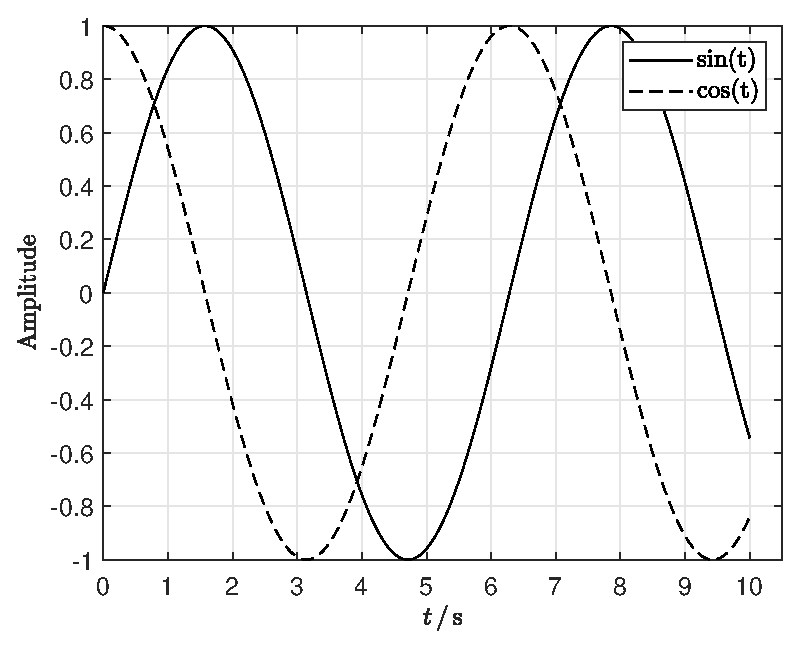
\includegraphics[width=0.62\textwidth]{img/Test_plot_1.eps}
    \caption[Kurzbeschreibung]{Abbildungsüberschrift}
    \label{fig:label}
\end{figure}

\section{Limitations and Identified Challenges}
